\chapter{Z Background Estimation}

We describe here two methods of estimating $Z\rightarrow\ell\ell$ backgrounds in our strong SUSY regions. The first method relies on the statistical manipulation of data-driven photon+jets backgrounds, and has been used in our previous analyses. We describe this method, and show that it is ill-suited to our current analysis due to violation of several underlying method assumptions. The second method we describe, based on the scaling of Z Monte Carlo samples to a \mindphijm\ control region for each signal and validation region, is the one we use for our current search. We show that this method replicates important features accurately, and is robust to theory systematic variations.

\section{Photon Method}

The photon+jets method is one which has been used before in both ATLAS and CMS~\cite{blah}, including in one of our previous analyses~\cite{blah}. In this method, we take photon+jets events from data and perform statistical manipulation to make them look like Z+jets events (Figure~\ref{fig:photon_to_Z}).

\begin{figure}[htbp]
    \centering
    \includegraphics[width=\textwidth]{Images/SUSY/photon_to_Z.png}
    \caption{A photon+jets event is made to resemble a Z+jets event by treating the photon as a Z boson of the same momentum, and by splitting it into two leptons.}
    \label{fig:photon_to_Z}
\end{figure}

The reason we do this is overcome limitations in QCD modelling in jets. That is, since most of the \MET\ in Z+jets events comes from the jets, and not from the Z or its lepton daughters, any analysis which involves \MET\ would benefit from using data-driven methods of estimating this particular background.

In this method, we can take a photon+jets event and treat the photon as a Z boson of the same \pt. We first "pseudo-split" the photon into two leptons. Second, we perform smearing adjustments on the leptons to simulate their relative measurement uncertainties. Finally, we scale the entire photon+jets \pt\ distribution to match the Z+jets \pt\ distribution.

\subsection*{Splitting}

To split the photon into two leptons, we first boost into the rest frame of the photon and perform the decay via a uniform angle sampling on the unit sphere. We then boost the daughter leptons back to the lab frame. In theory, this would allow us to replicate the lepton distributions in our Z+jets background.

However, here we run into our first problem. There are differences in the $\eta$ distributions of photons and Z bosons (Figure~\ref{fig:Z_photon_eta}). As well, there are $\eta$ acceptance distributions for each type of lepton. As such, we have to perform a reweighting in lepton $\eta$ to get the photon "pseudo-split" leptons to match up. However, this is made more difficult by the $|\eta|<2.37$ requirement on photons, as well as the $\eta$ acceptance gaps.

\begin{figure}[htbp]
    \centering
    \includegraphics[width=0.45\textwidth]{Images/SUSY/Z_eta.png}
    \includegraphics[width=0.45\textwidth]{Images/SUSY/photon_eta.png}
    \caption{Z $\eta$ distribution (left) vs. photon $\eta$ distribution.}
    \label{fig:Z_photon_eta}
\end{figure}

By having to use low-$\eta$ photons to simulate high-$\eta$ Z+jets events, we get slight unavoidable differences in lepton distributions. These problems caused some issues in final \MET\ distributions, since the leptons were used to perform \MET\ smearing (as will be described next).

\subsection*{Smearing}

The resolution smearing step is to account for the fact that photons and leptons have different measurement resolutions within our detector. In particular, there is significant mismeasurement of muons at high \pt, which produces a contribution to \MET\ in the propagation direction of the muon. Though most \MET\ in our Z/$\gamma$+jets events is taken to be coming from the jets, these leptonic contributions cause an effect which must be corrected for.

To simplify calculations, we treat lepton propagation as mostly being in the direction of Z/$\gamma$ propagation. Thus our smearing method only affects \MET\ in the direction parallel to the direction of Z/$\gamma$ propagation (\METl), and not in the transverse direction (\METt). To apply smearing, we look at \METl\ in slices of \pt\ for both photon and Z events in MC. For each bin, we calculate the differences in mean and standard deviation for the photon and Z distributions.

For electrons we apply a shift in mean \METl\ for each event, and for muons we apply both a shift in mean and an additional smearing in resolution based on sampling from a Gaussian of the given standard deviation. Comparisons of photon and Z \METl\ distributions after smearing in various \pt\ slices can be seen in Figure~\ref{fig:Z_photon_eta}.

\begin{figure}[htbp]
    \centering
    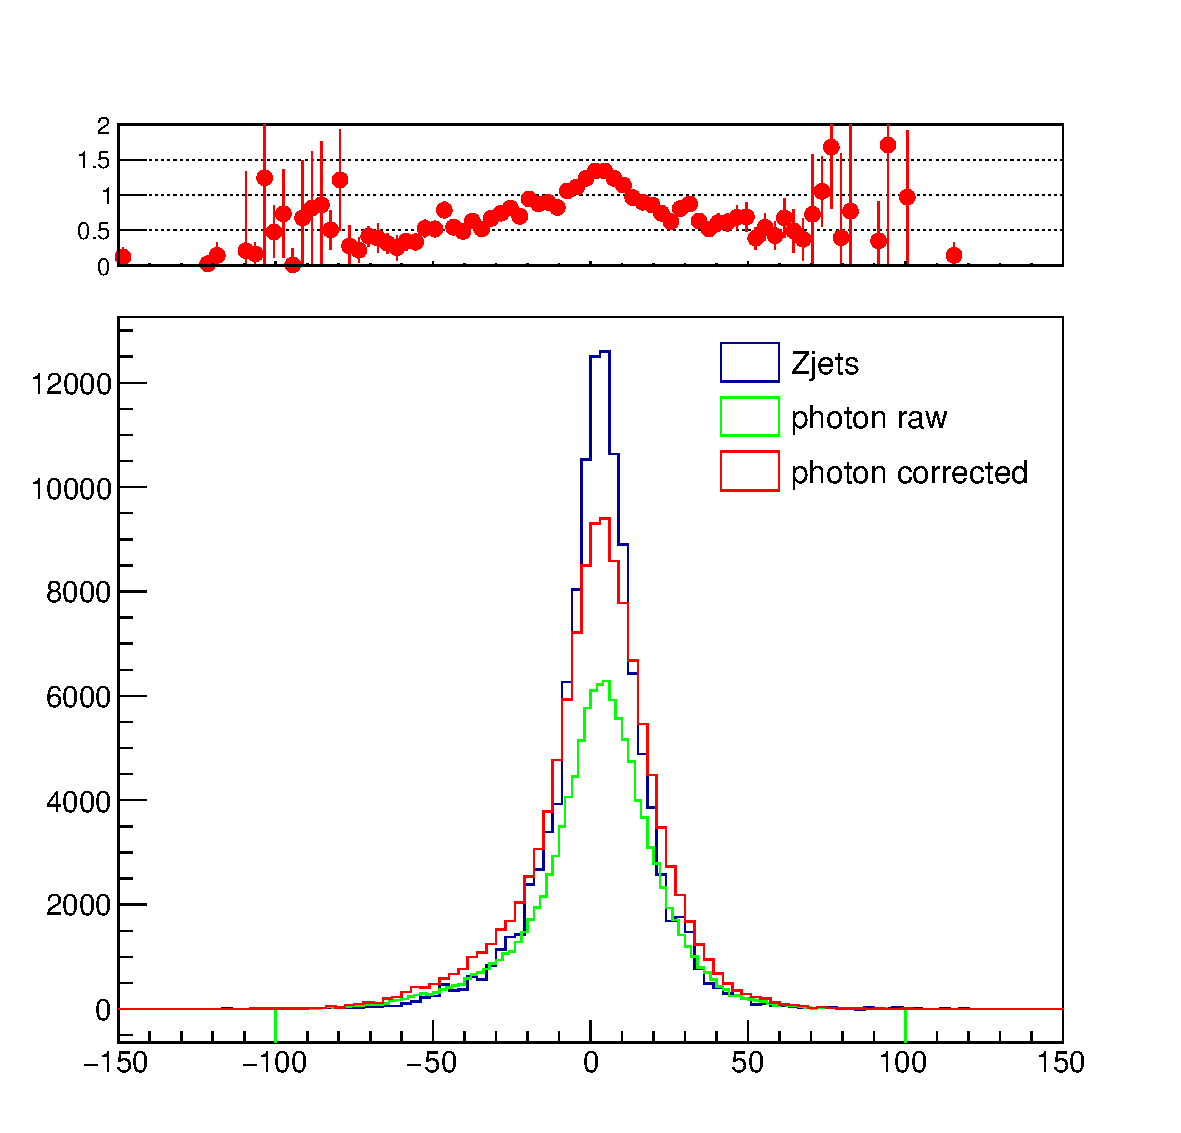
\includegraphics[width=0.45\textwidth]{Images/SUSY/METl_bin_5.pdf}
    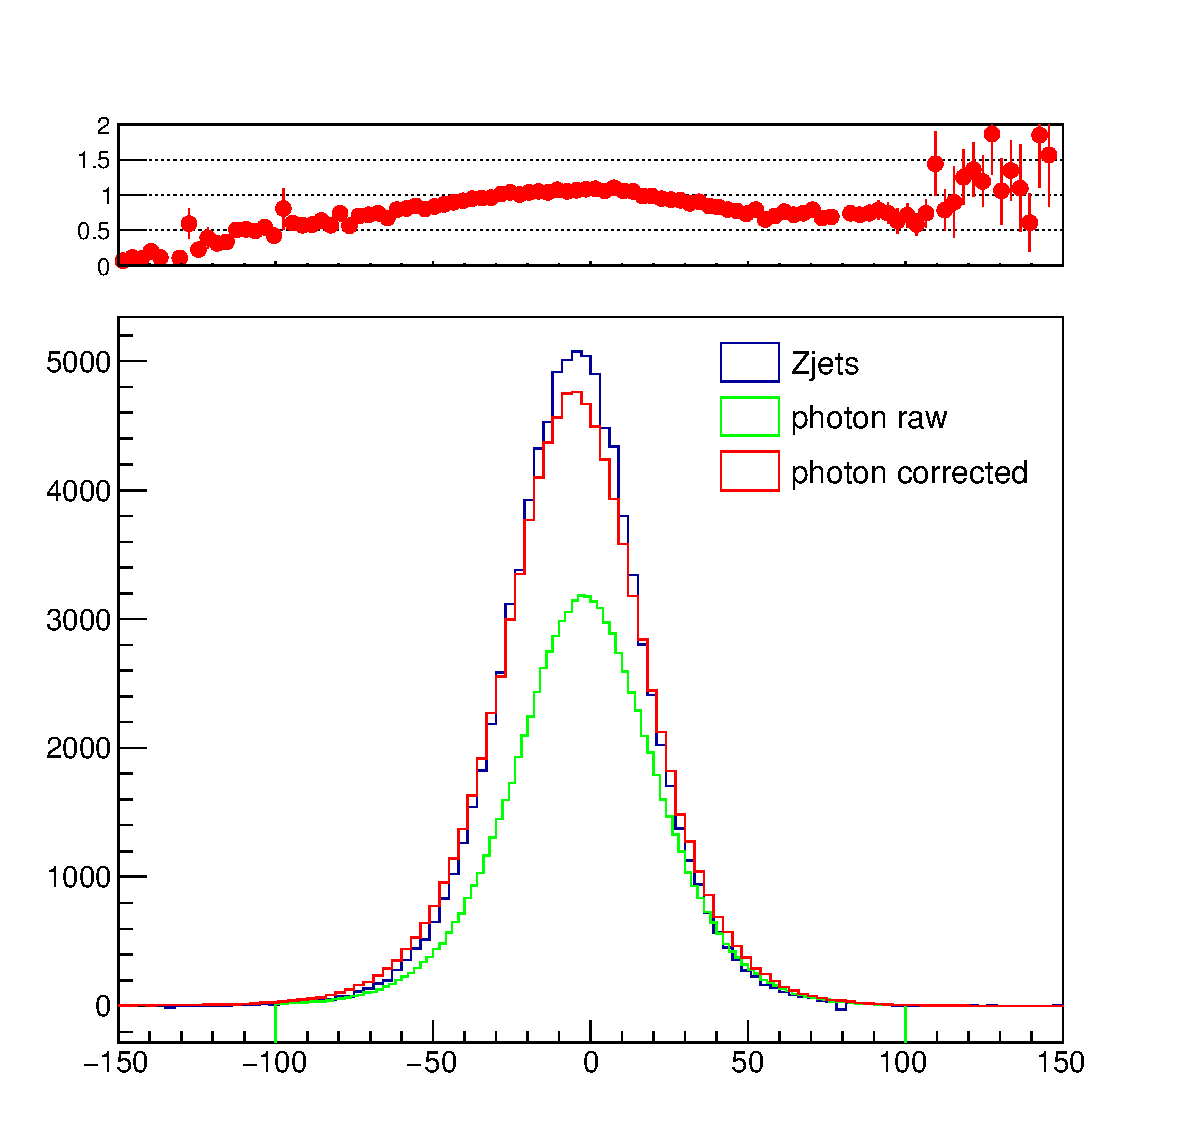
\includegraphics[width=0.45\textwidth]{Images/SUSY/METl_bin_16.pdf}
    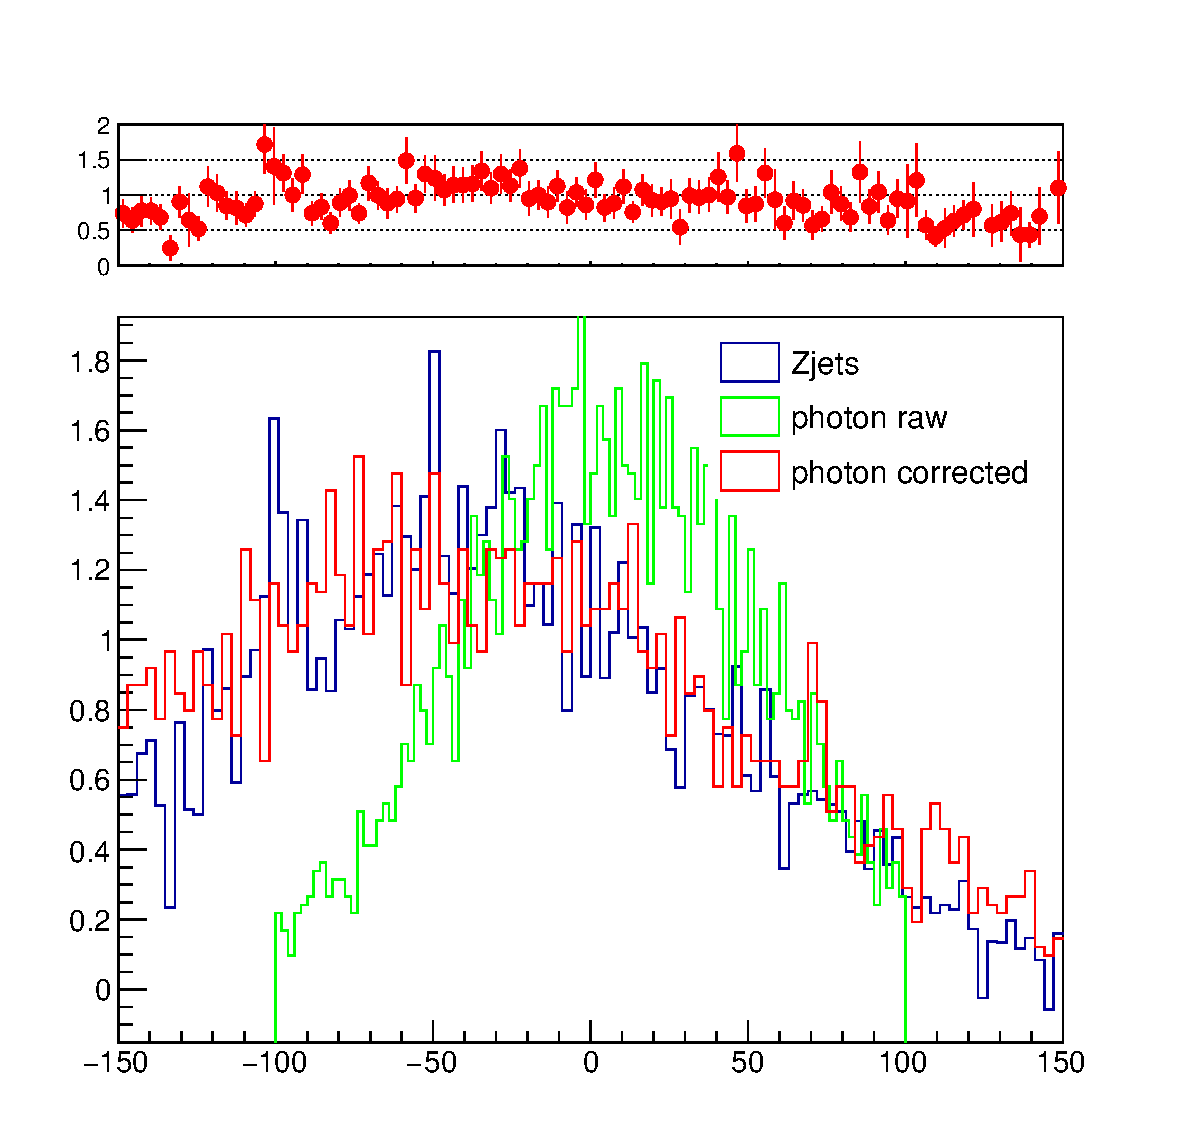
\includegraphics[width=0.45\textwidth]{Images/SUSY/METl_bin_21.pdf}
    \caption{\METl\ comparisons between Z+jets (in the $\mu\mu$ channel) and smeared photon+jets events in a low-\pt\ bin (left), a medium-\pt\ bin (right), and a high-\pt\ bin (bottom). Scaling has been applied to smeared photons.}
    \label{fig:Z_photon_eta}
\end{figure}

These \pt-binned \METl\ comparisons reveal a problem. Though \METl\ is replicated well at high \pt, turning a photon distribution that looked nothing like the Z distribution into something fairly close, the effect is not so good at low \pt. In fact, at low \pt\ we see that the photon resolution started off worse than the muon resolution, violating one of the assumptions of our method. There, the smearing method allowed us to mean-shift to better match the Z+jets \METl\ distribution, but could not simulate the required improvement in resolution.

The overall result of the smearing method can be seen in Figure~\ref{fig:Z_photon_eta_total}. We see that though the photon \METl\ distribution has improved, it still does not match well with the Z+jets distribution. In particular, there is a skew issue which comes from the facts that \METl\ means shift leftward as \pt\ increases, and that smearing performs worse at low \pt. This problem ended up causing mismodeling issues with the \MET\ variables.

\begin{figure}[htbp]
    \centering
    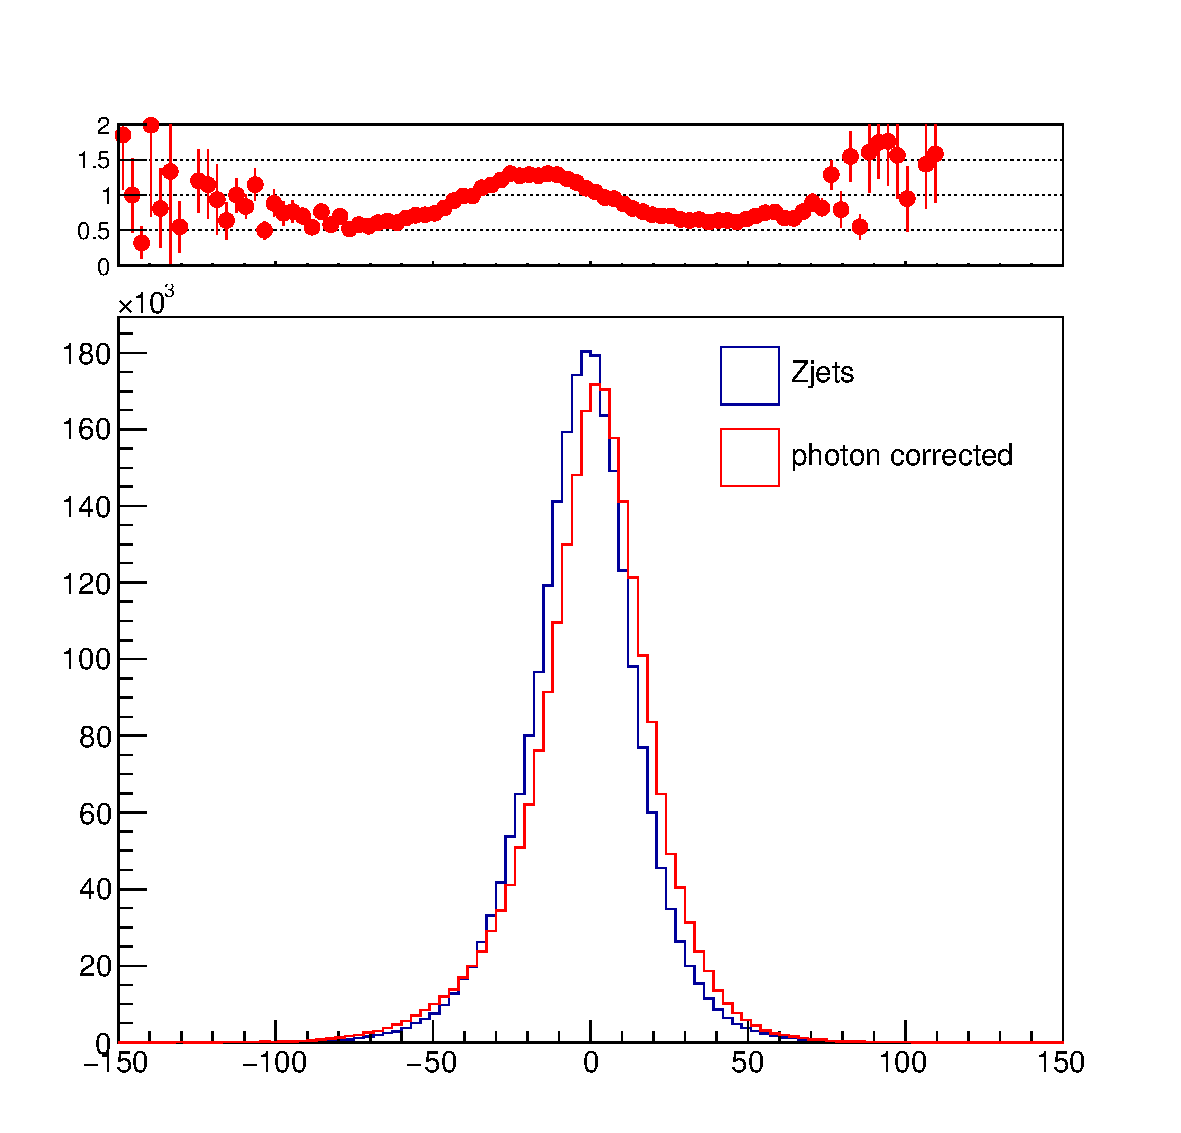
\includegraphics[width=0.45\textwidth]{Images/SUSY/METl_total.pdf}
    \caption{\METl\ comparisons between all Z+jets and smeared photon+jets events.}
    \label{fig:Z_photon_eta_total}
\end{figure}

\subsection*{Reweighting}

Next, we take into account the fact that photon and Z processes are produced with different \pt\ distributions. We correct for this by reweighting photon events in \pt\ bins in order to match the distribution seen in Z events.

To do this, we look at \pt\ slices in an inclusive region ($>=2$ leptons, $>=2$ jets). We compare yields for photons vs. Z, as determined by data minus all other relevant processes. In each \pt\ bin, we scale photon events by the ratio of photons vs. Z yields. Comparisons of photon vs. Z \ptll\ distributions both before and after reweighting are shown in Figure~\ref{fig:reweighting}.

\begin{figure}[hbtp]
    \centering
    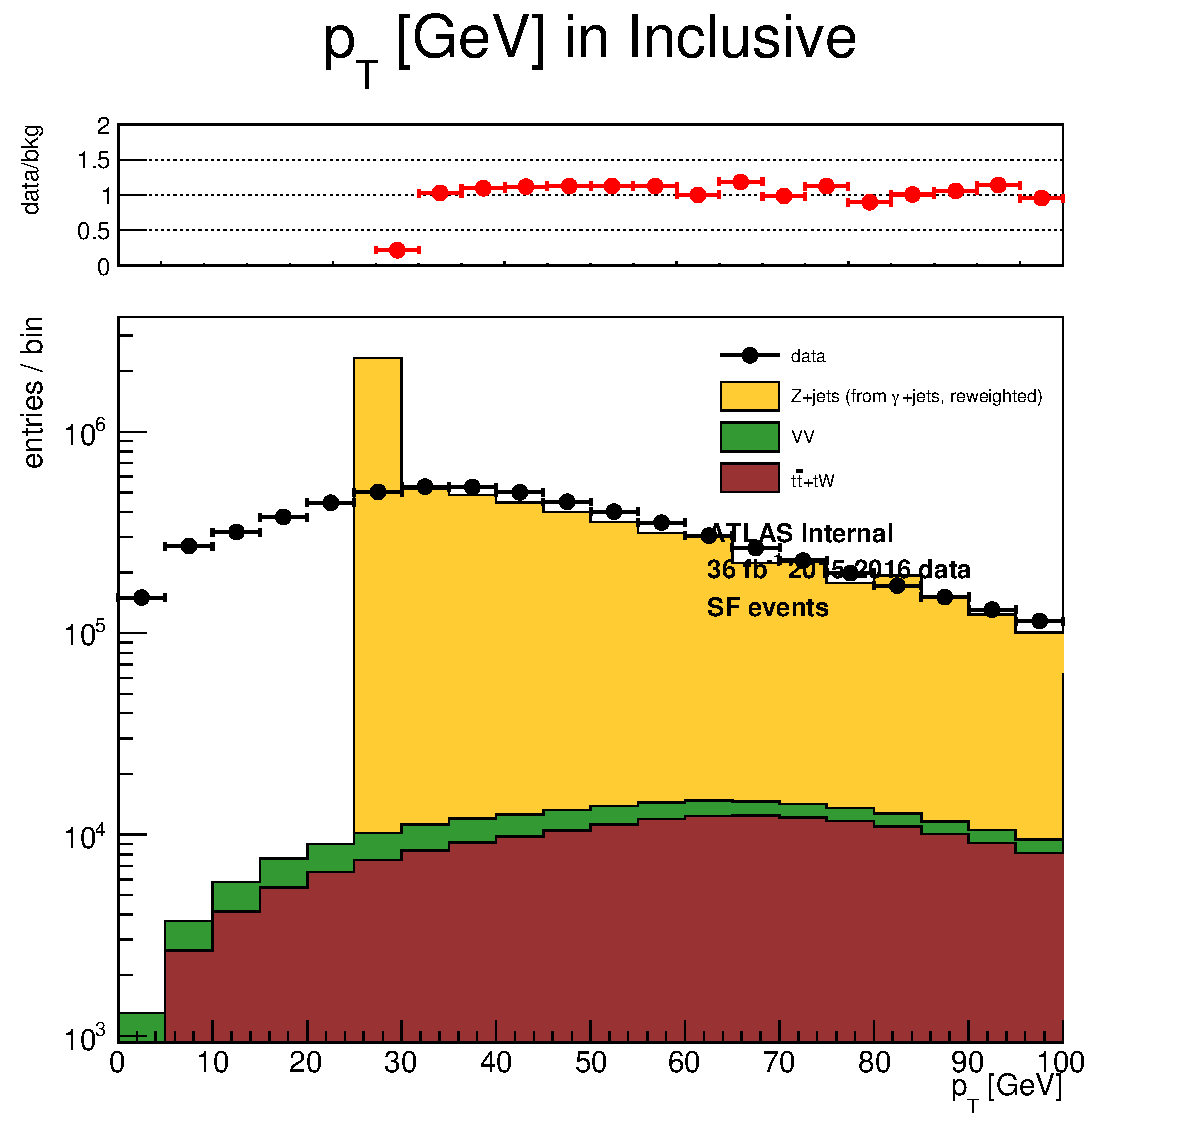
\includegraphics[width=0.7\textwidth]{Images/SUSY/ptll_distributions.pdf}
    \caption{Data \pt\ distribution in an inclusive region, along with diboson MC, ttbar MC, and reweighted data photons. We see that the photon \pt\ does not extend below 25 GeV.}
    \label{fig:reweighting}
\end{figure}

However, this leads to our third problem. We see in the plot that the photon \pt\ range does not extend all the way down. This is due to different availabilities of photon and Z triggers. Lacking the low-\pt\ photon information means that a lot of the soft lepton events would be inaccurately modelled by this method.

\subsection*{Examining Other Assumptions}

We have seen several problems already which make the photon+jets method problematic in this analysis. We can see \MET\ features as calculated via this method in Figure~\ref{fig:photon_method_MET}. We see that the modelling here can definitely be better.

\begin{figure}[hbtp]
    \centering
    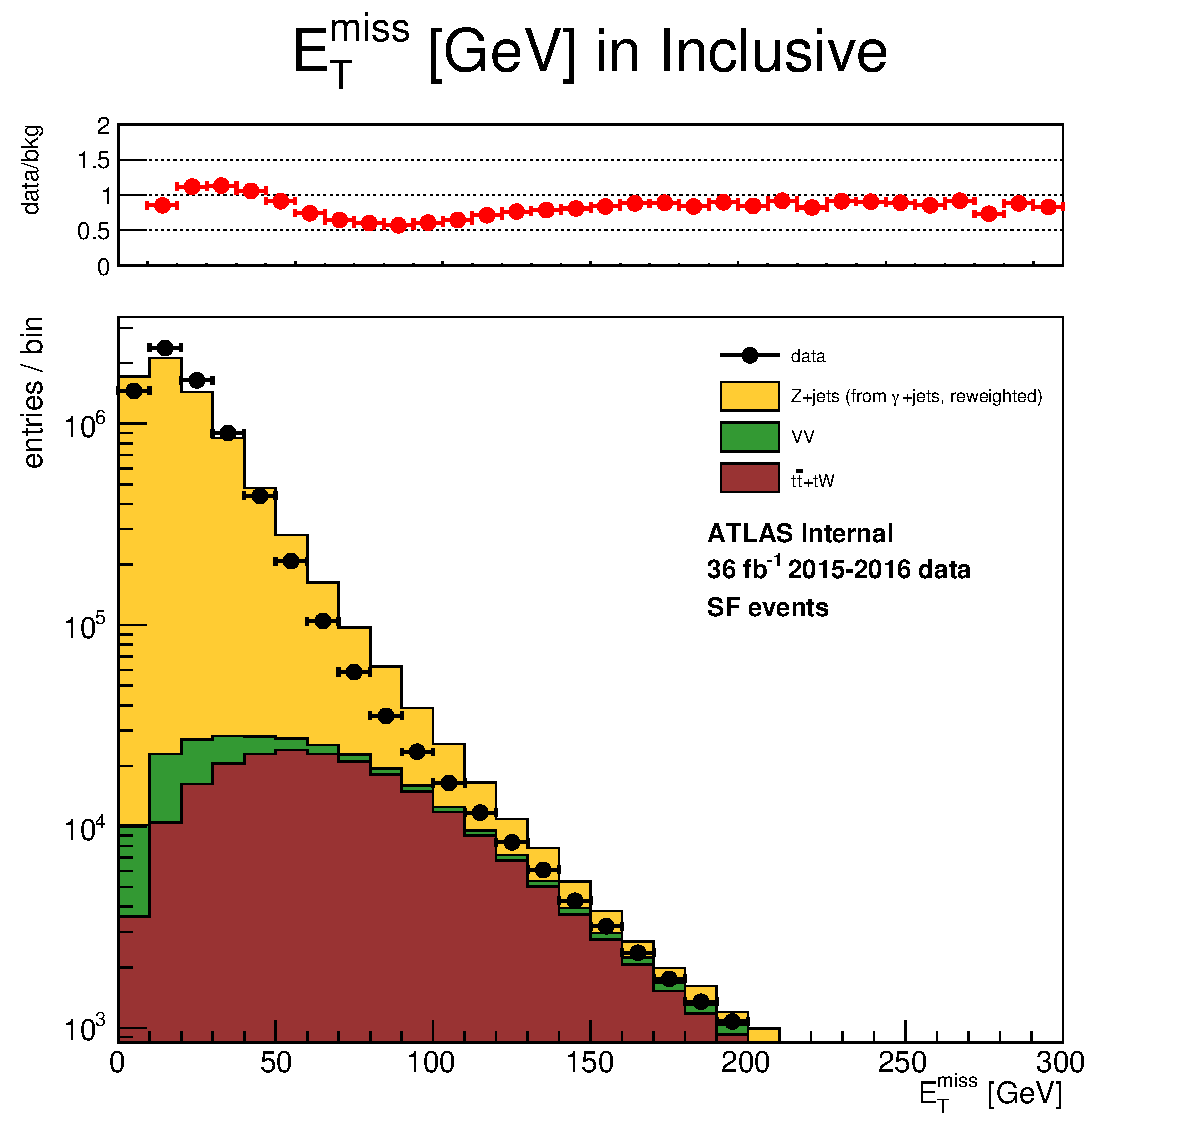
\includegraphics[width=0.45\textwidth]{Images/SUSY/photon_method_MET.pdf}
    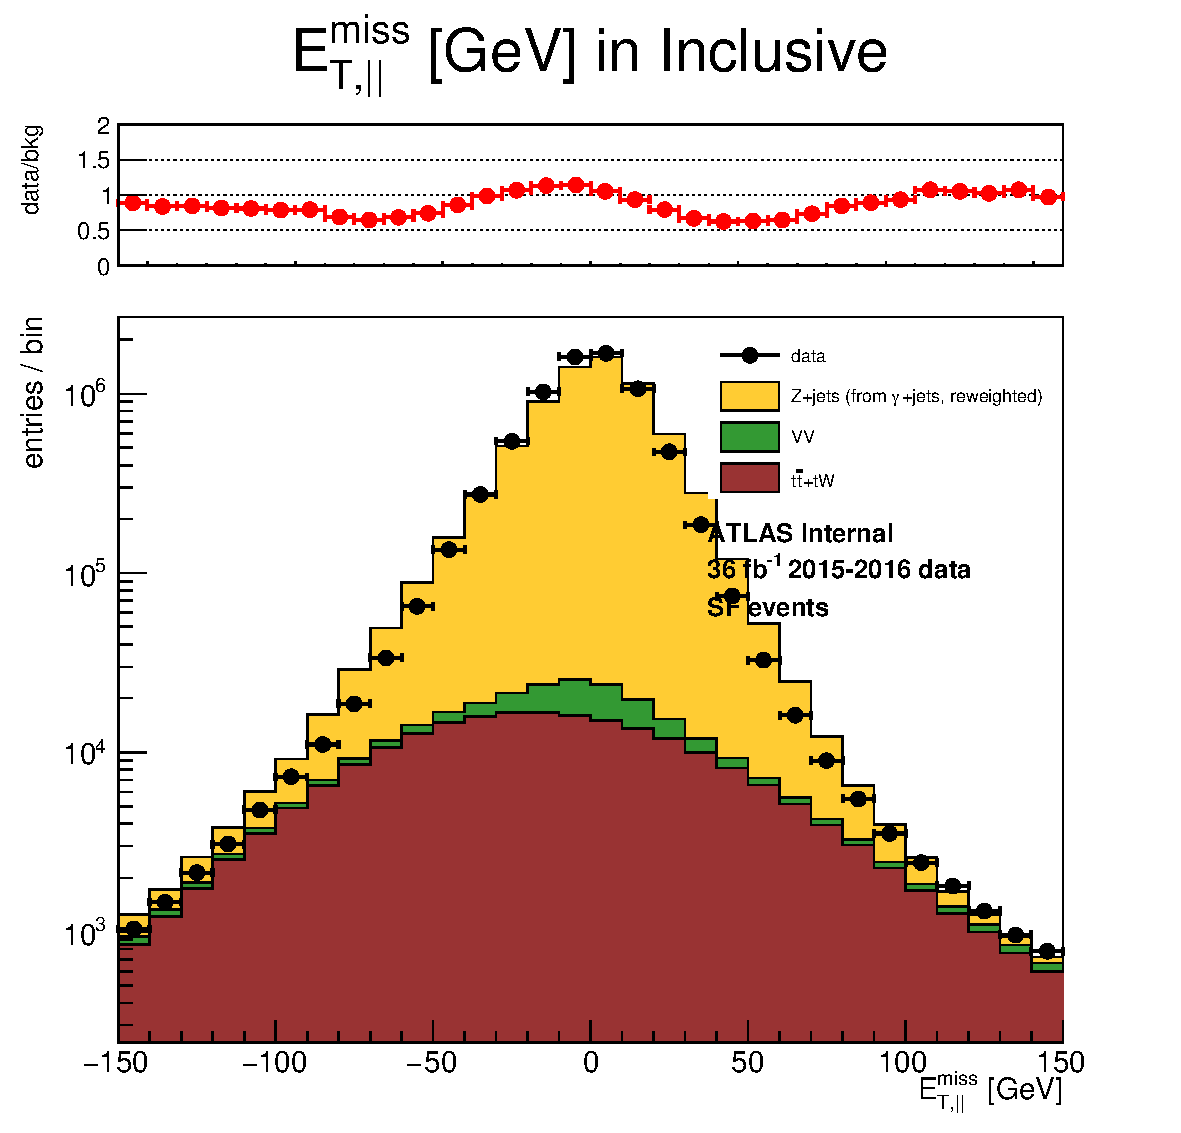
\includegraphics[width=0.45\textwidth]{Images/SUSY/photon_method_METl.pdf}
    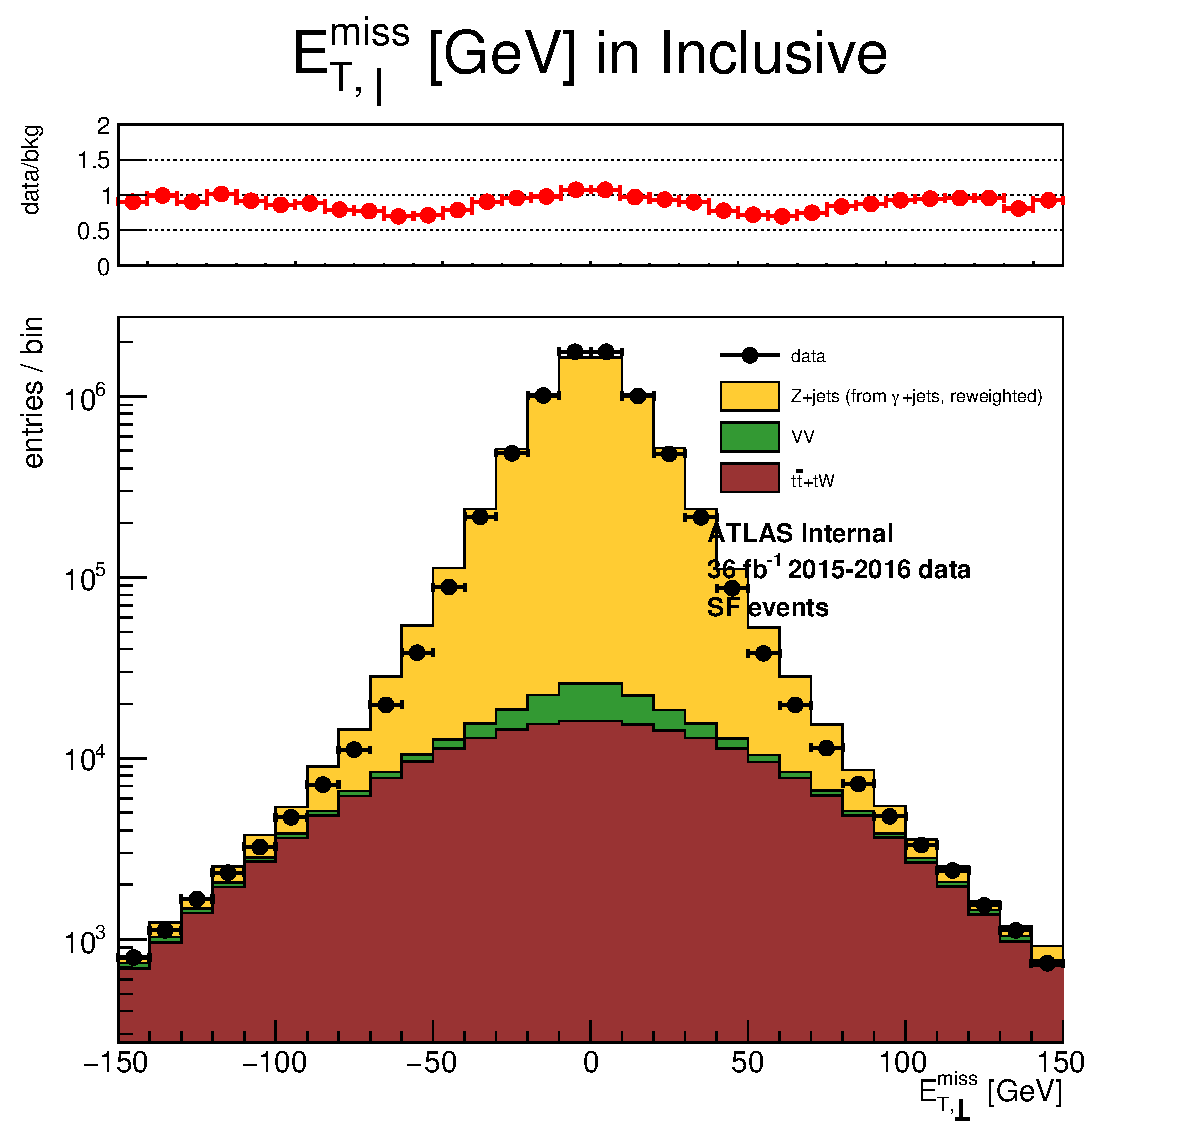
\includegraphics[width=0.45\textwidth]{Images/SUSY/photon_method_METt.pdf}
    \caption{\MET\ distributions, as determined by the data-driven photon+jets method. We have (left) \MET, (right) \METl, and (bottom) \METt.}
    \label{fig:photon_method_MET}
\end{figure}

However, aside from these issues, we can identify some problems in our initial assumptions as well. Our entire method hinges on the idea that \MET\ in Z/$\gamma$+jets events comes mostly from jets, not from the bosonic elements. We examine this assumption by plotting \mindphijm\ and \dphiptllmet. If \MET\ does indeed come mostly from jets, then we would expect the distribution of \mindphijm\ to be peaked around $\phi$ of 0 and $\pi$, and we would expect that of \dphiptllmet\ to be mostly flat.

The \mindphijm\ and \dphiptllmet\ distributions for Z and for photon are shown in Figures~\ref{fig:Z_distributions} and~\ref{fig:photon_distributions}, given the baseline preselections for the photon method. We see that the initial assumption is significantly violated for both processes. For these reasons, we decided to investigate a different method of Z background estimation.

\begin{figure}[hbtp]
    \centering
    \includegraphics[width=0.45\textwidth]{Images/SUSY/Z_dphijm.png}
    \includegraphics[width=0.45\textwidth]{Images/SUSY/Z_dphipm.png}
    \caption{\mindphijm\ (left) and \dphiptllmet\ (right) distributions for Z MC, given baseline preselections ($>=2$ leptons, leading leptons OS, $>=1$ jet, \ptll$>25$).}
    \label{fig:Z_distributions}
\end{figure}

\begin{figure}[hbtp]
    \centering
    \includegraphics[width=0.45\textwidth]{Images/SUSY/photon_dphijm.png}
    \includegraphics[width=0.45\textwidth]{Images/SUSY/photon_dphipm.png}
    \caption{\mindphijm\ (left) and \dphiptllmet\ (right) distributions for photon data, given baseline preselections (no leptons, $>=1$ jet, \ptll$>25$).}
    \label{fig:photon_distributions}
\end{figure}

\section{Z MC Method}

Due to all of the problems listed in the last section, we decided to take a look at Z MC again. Luckily, it appeared that with recent Monte Carlo sample generation updates, many of the problems previously seen with QCD modelling were no longer an issue.

We developed a new MC-based method for Z background estimation (dubbed the \mindphijm\ method), and performed systematics checks as well as visual comparisons of various \MET\ and jet features. These checks revealed that Z MC using the new method modelled \MET\ variables well.

\subsection*{dPhi Scaling Method}

In this method, we define a new control region for each of our signal and validation regions. Where our normal regions have a \mindphijm$>0.4$ cut, our control regions have an opposite \mindphijm$<0.4$ cut. This new cut maximizes the Z+jets contribution in the region by looking specifically for events where \MET\ is coming from jets.

Though we saw previously that there are a significant percentage of Z+jets events where \MET\ is not aligned with the jets, the converse statement still appears to be valid. That is, events where \MET\ aligns with jets are disproportionately coming from Z+jets processes. We can validate this statement by looking at Z yields vs. yields from other processes in the upcoming tables.

For each control region, we find a scaling factor for Z MC such that the sum of all background yields in the control region equals the data yield. That is, the scale factor is equal to the total yield of data minus non-Z backgrounds, divided by Z yield. The scaling factor is then used to scale Z MC in the normal region to produce the final predicted yield.

\subsection*{Method Validation}

We first demonstrate the validity of the method by defining a loose region called VRZ, which is dominated by Z+jets events. In this region we use MC to estimate all backgrounds. VRZ has exactly two same-flavor leptons and at least two jets, no b-tagged jets, and \ptll$>40$. VRZ also has the \mindphijm$<0.4$ cut common to all our regions.

We check the resulting \MET, \mindphijm, and \dphiptllmet\ shapes in VRZ. The data vs. MC \MET distribution in VRZ is presented in Figure~\ref{fig:VRZ_MET}, while \mindphijm\ and \dphiptllmet\ are shown both inclusively and in four \MET\ bins (0-50 GeV, 50-100 GeV, 100-150 GeV, and 150-200 GeV) in Figures~\ref{fig:VRZ_dPhi2JetMET} and~\ref{fig:VRZ_dPhiPtllMET}. As demonstrated in these figures, the MC provides good modeling of relevant quantities.

\begin{figure}[htbp]
\centering
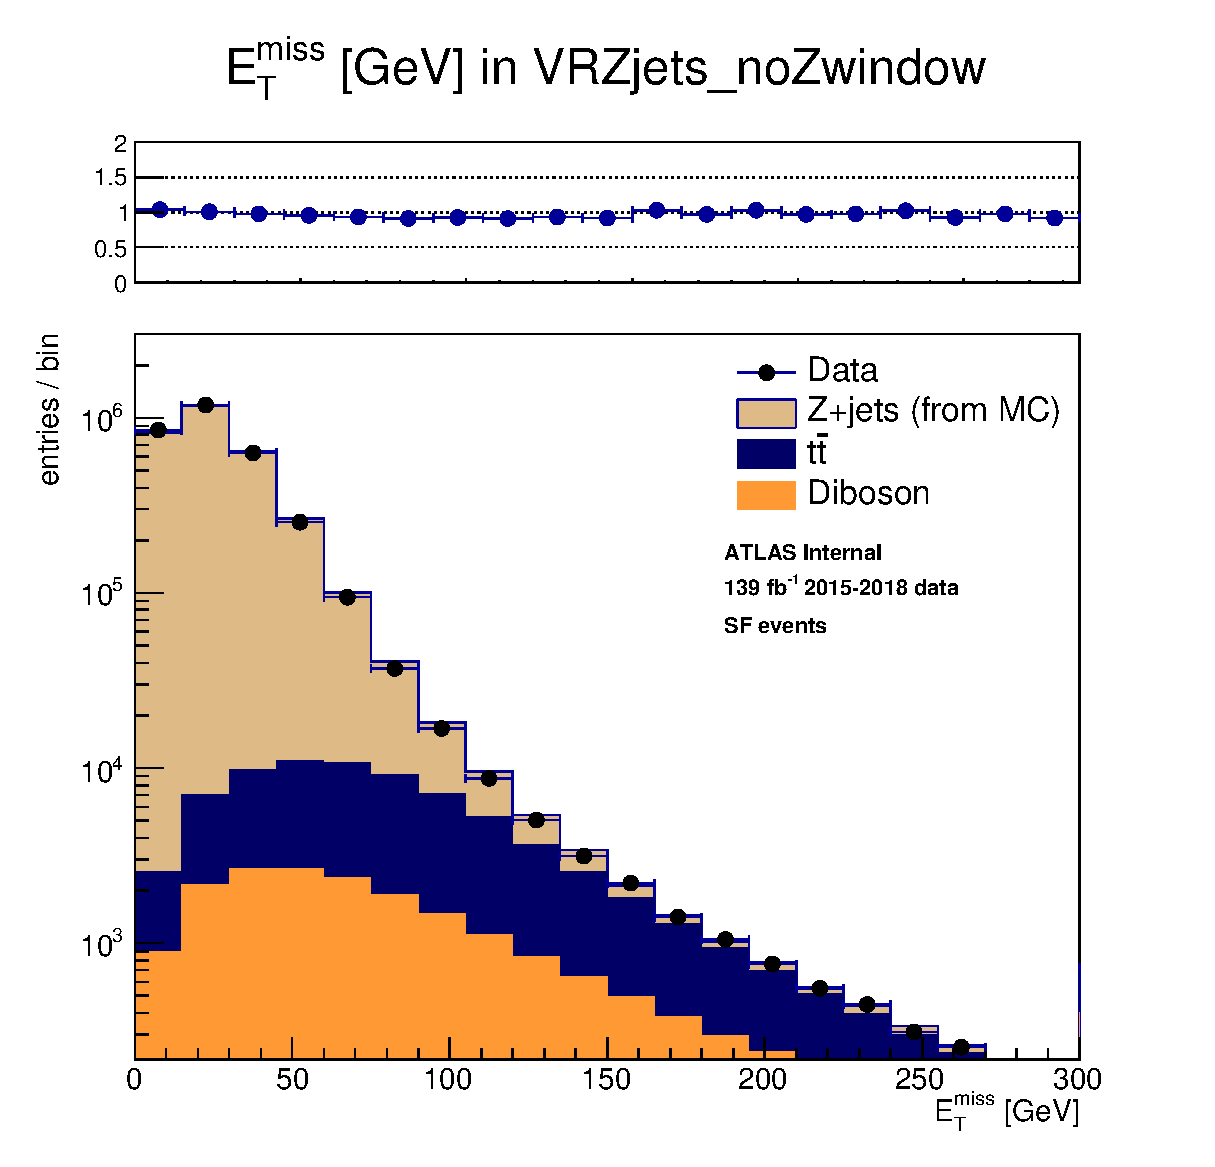
\includegraphics[width=0.7\textwidth]{Images/SUSY/reweight_Ptll_all_SF_met_Et_VRZ.eps}
\caption{\MET\ in the VRZ validation region. A scaling factor has been applied based on using the \mindphijm\ method in the corresponding control region. The y-axis is on a log scale.}
\label{fig:VRZ_MET}
\end{figure}

\begin{figure}[htbp]
\centering
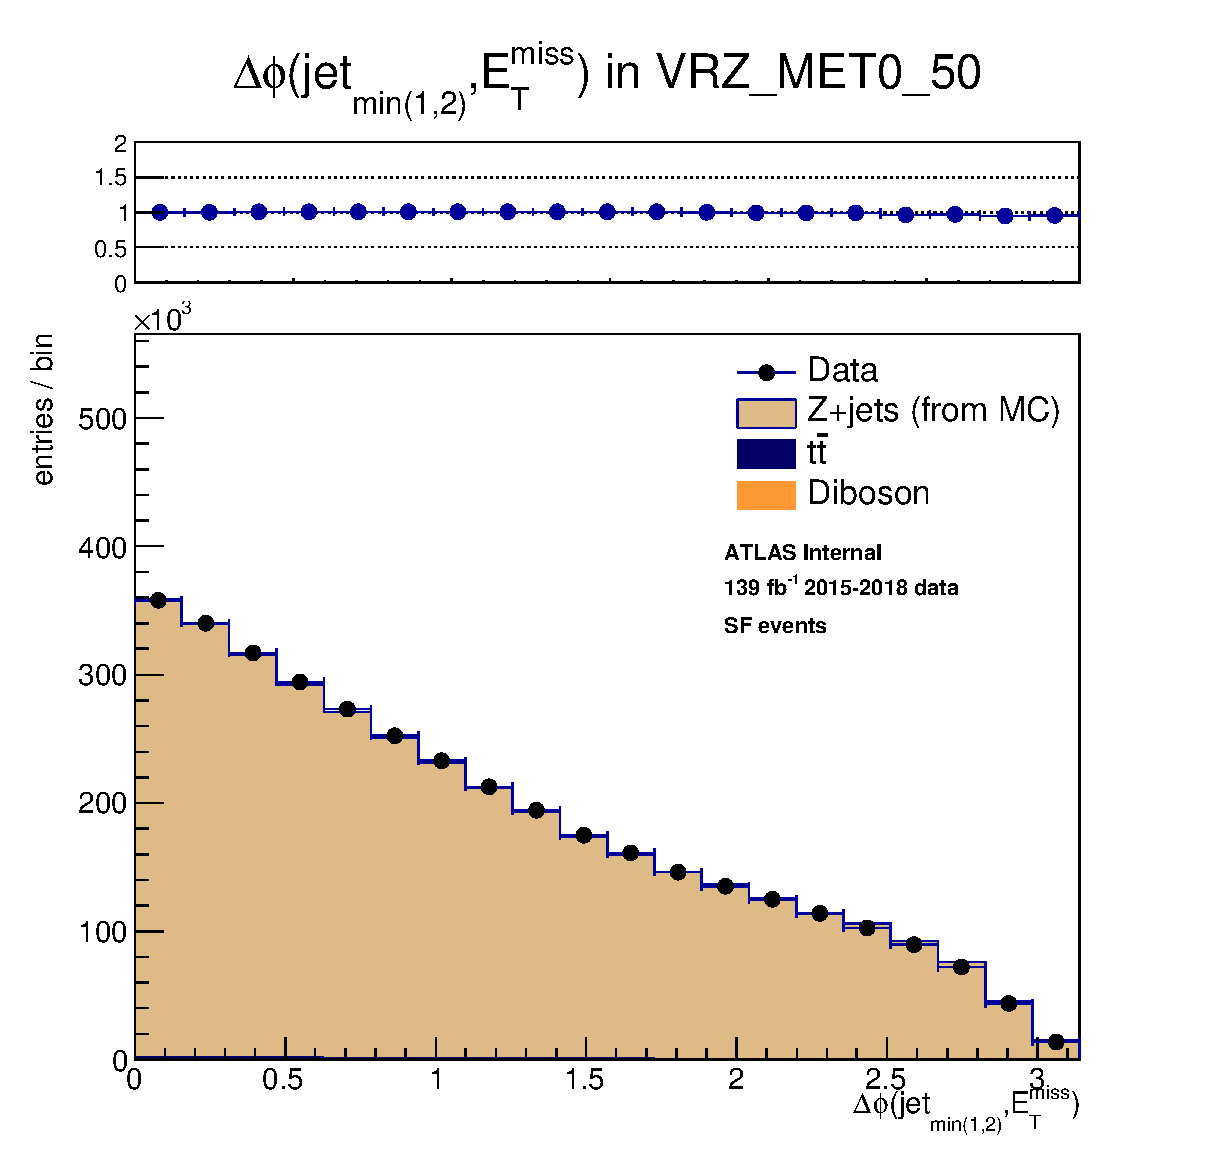
\includegraphics[width=0.45\textwidth]{Images/SUSY/reweight_Ptll_all_SF_minDPhi2JetsMet_VRZ_MET0_50.eps}
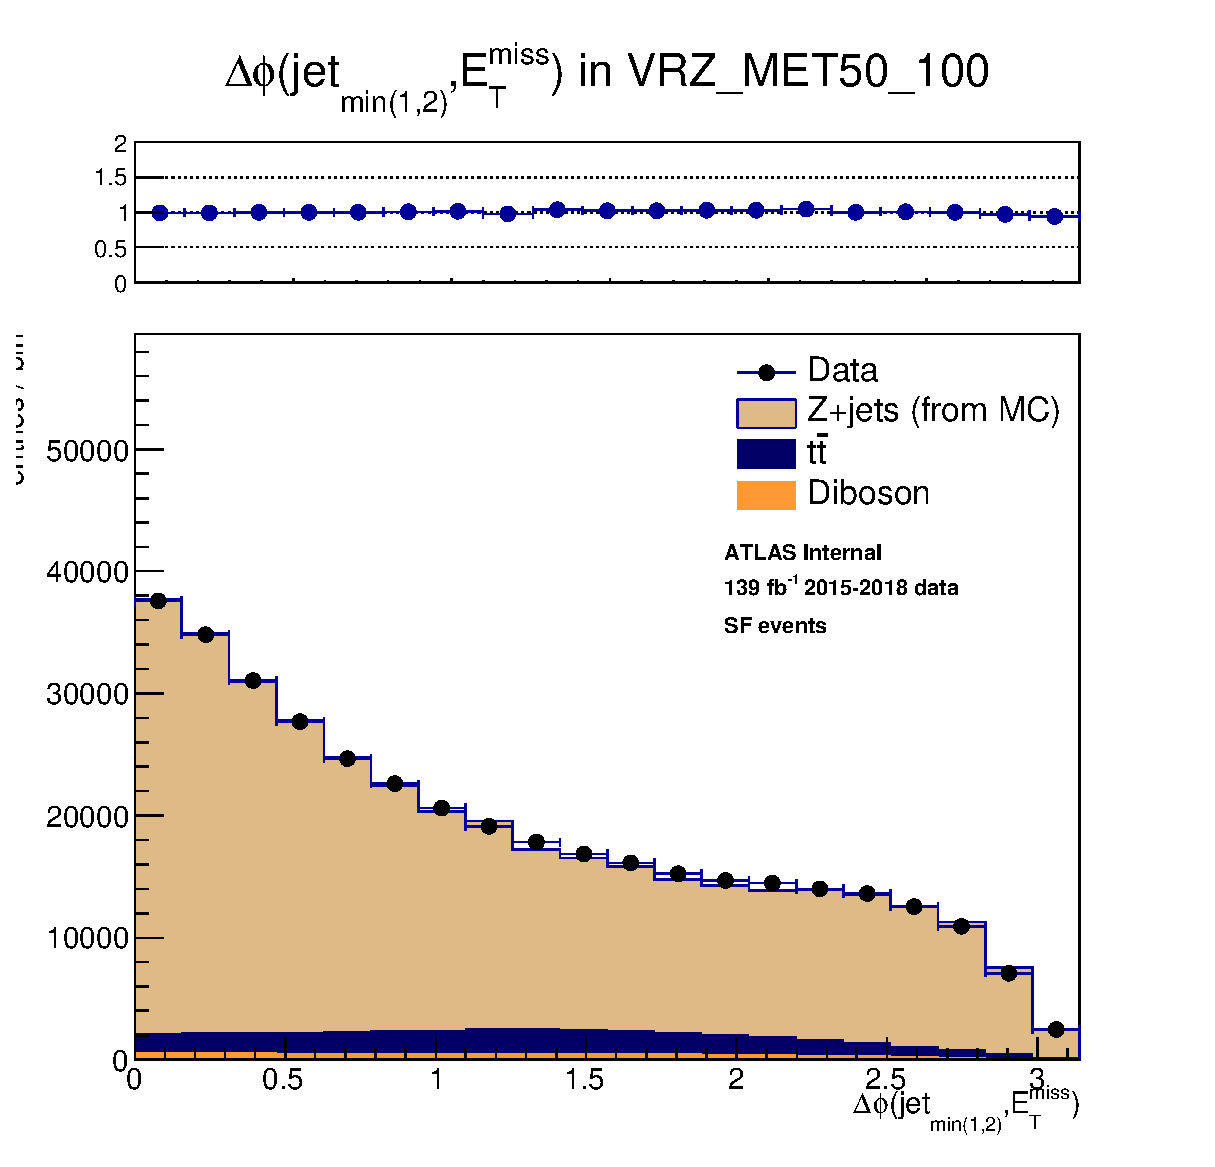
\includegraphics[width=0.45\textwidth]{Images/SUSY/reweight_Ptll_all_SF_minDPhi2JetsMet_VRZ_MET50_100.eps}
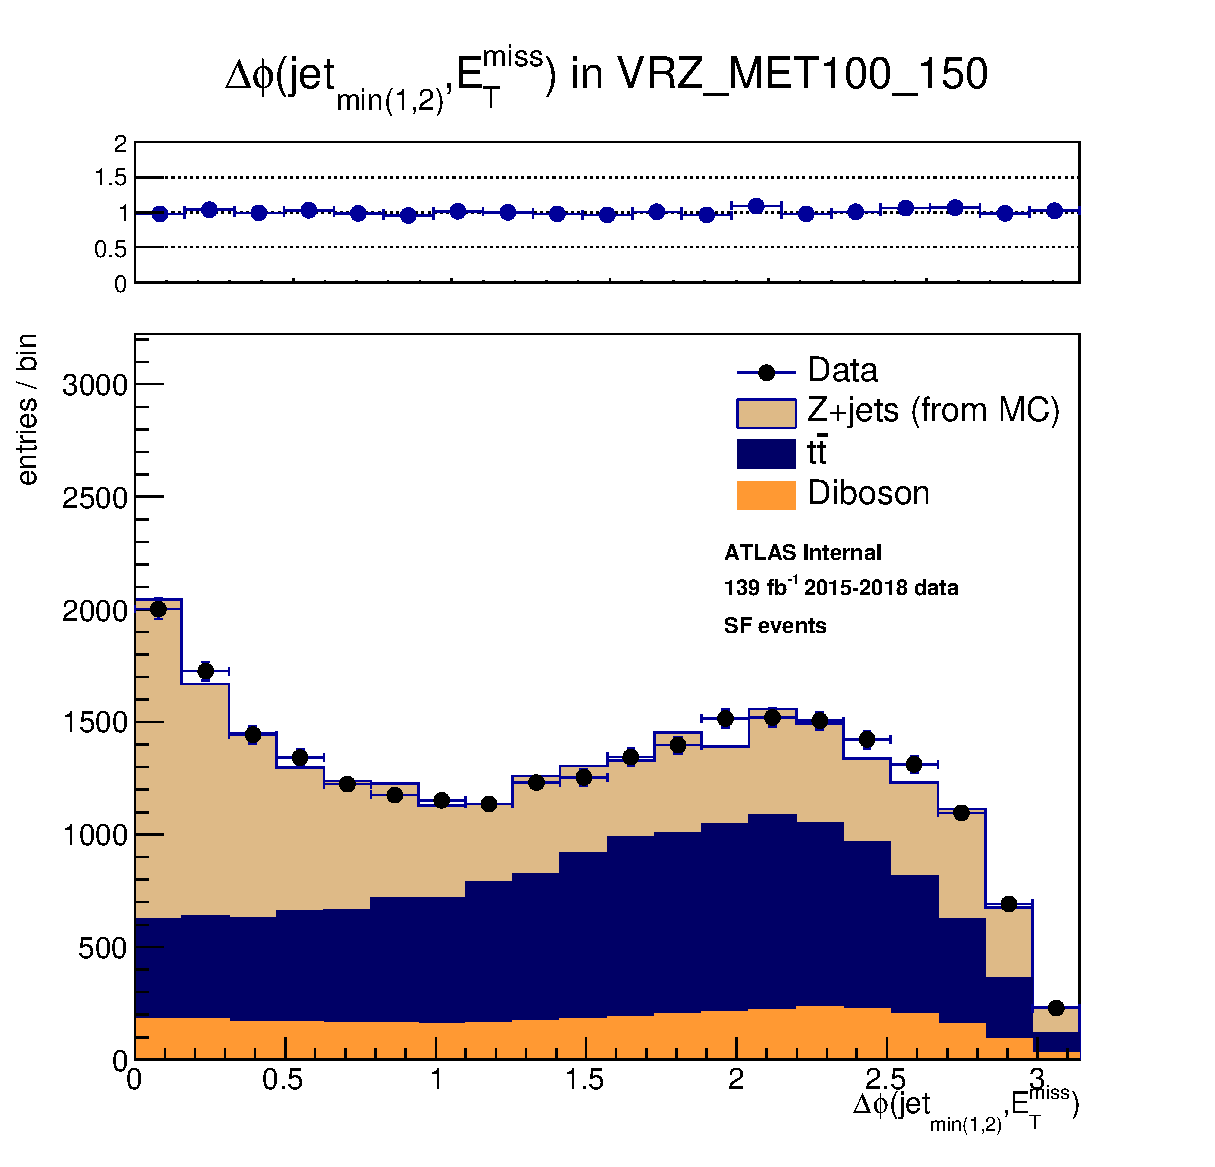
\includegraphics[width=0.45\textwidth]{Images/SUSY/reweight_Ptll_all_SF_minDPhi2JetsMet_VRZ_MET100_150.eps}
\includegraphics[width=0.45\textwidth]{Images/SUSY/reweight_Ptll_all_SF_minDPhi2JetsMet_VRZ_MET150_200.eps}
\includegraphics[width=0.45\textwidth]{Images/SUSY/reweight_Ptll_all_SF_minDPhi2JetsMet_VRZ.eps}
\caption{\mindphijm\ in VRZ, both inclusively (bottom) and in various MET bins.}
\label{fig:VRZ_dPhi2JetMET}
\end{figure}

\begin{figure}[htbp]
\centering
\includegraphics[width=0.45\textwidth]{Images/SUSY/reweight_Ptll_all_SF_dPhiPllMet_VRZ_MET0_50.eps}
\includegraphics[width=0.45\textwidth]{Images/SUSY/reweight_Ptll_all_SF_dPhiPllMet_VRZ_MET50_100.eps}
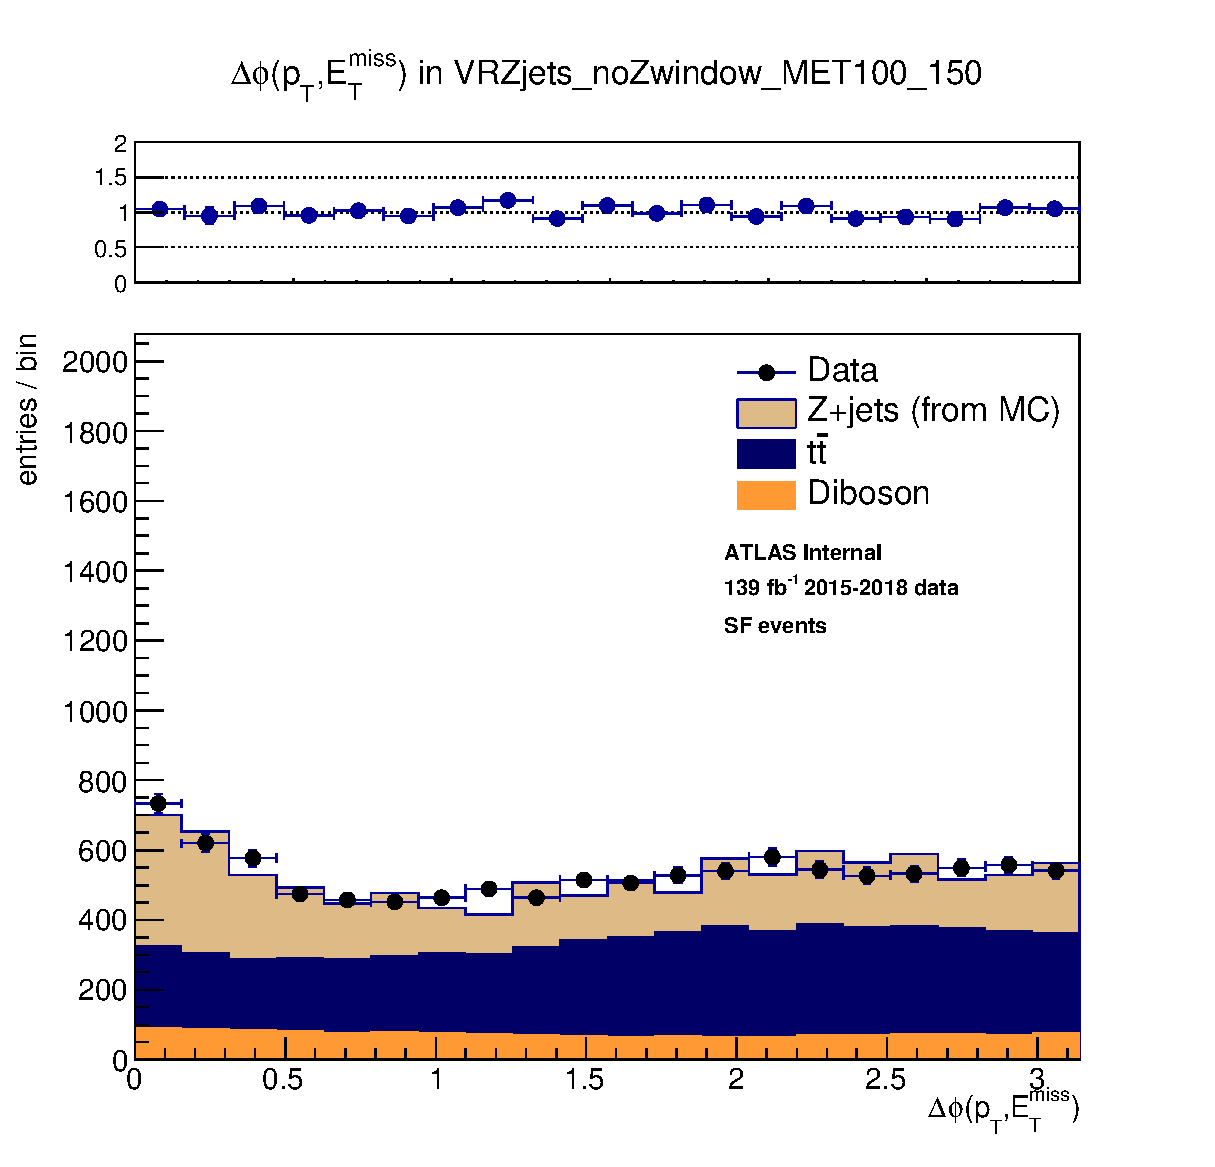
\includegraphics[width=0.45\textwidth]{Images/SUSY/reweight_Ptll_all_SF_dPhiPllMet_VRZ_MET100_150.eps}
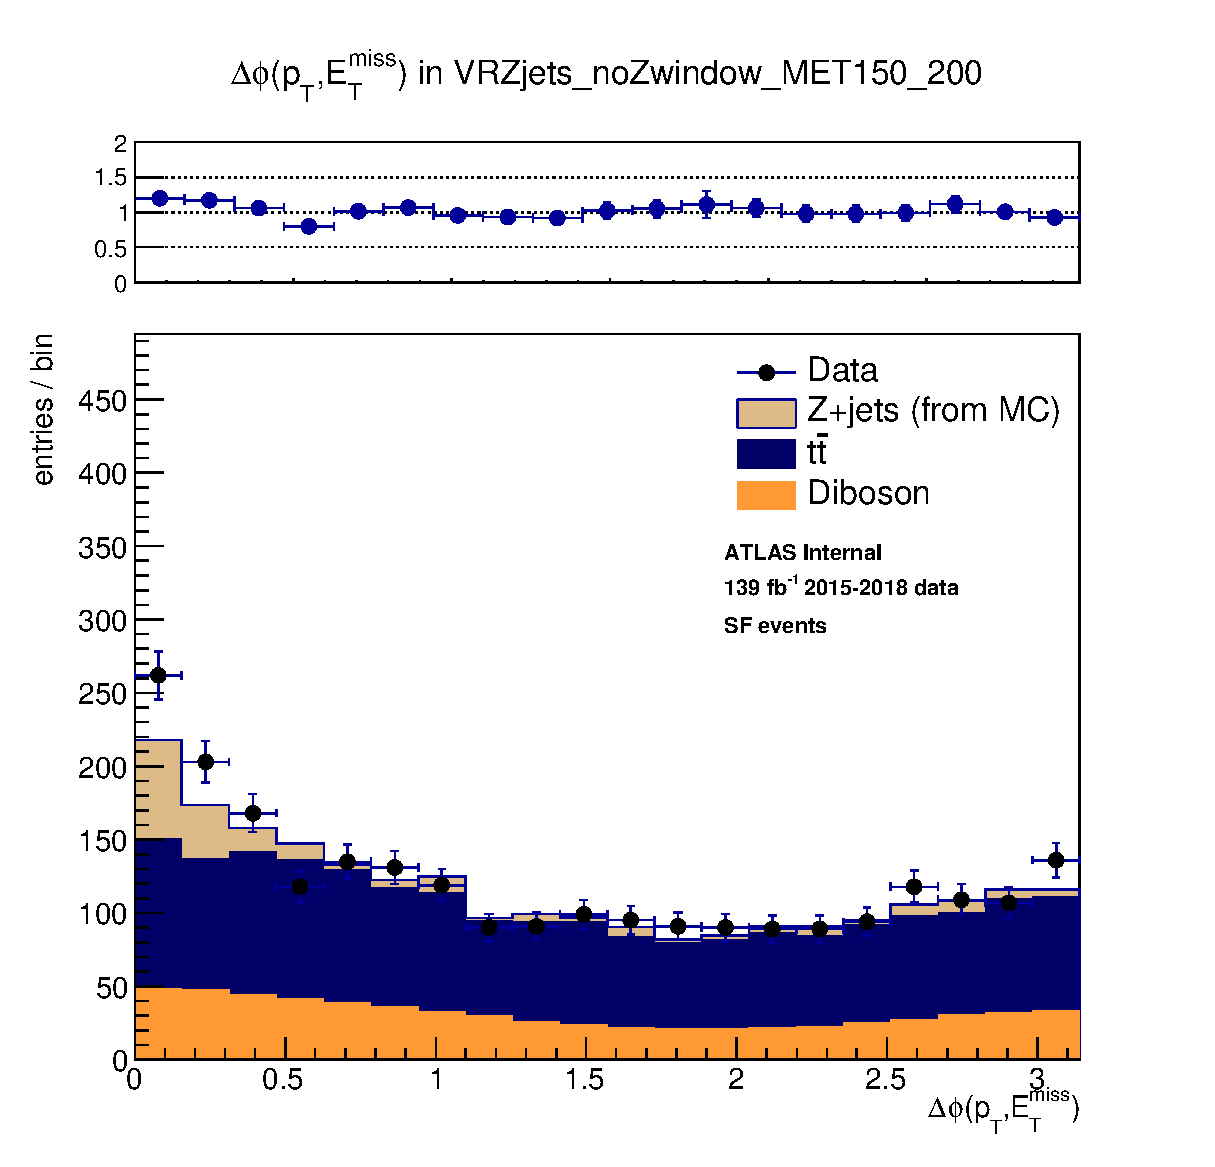
\includegraphics[width=0.45\textwidth]{Images/SUSY/reweight_Ptll_all_SF_dPhiPllMet_VRZ_MET150_200.eps}
\includegraphics[width=0.45\textwidth]{Images/SUSY/reweight_Ptll_all_SF_dPhiPllMet_VRZ.eps}
\caption{\dphiptllmet\ in VRZ, both inclusively (bottom) and in various MET bins.}
\label{fig:VRZ_dPhiPtllMET}
\end{figure}

\subsection*{Scale Factors and Yields}

The scale factors obtained via this method are shown in Table~\ref{tab:ZMC_SF} for each strong signal and validation region. Statistical uncertainties are calculated based on the number of events in each region.

\begin{table}[htbp]
\begin{center}
\begin{tabular}{l|r}
    \hline
    \hline
    Region & Z+jets Scale Factor \\
    \hline
    VRZ & $1.076\pm0.003$ \\
    VRZ + \MET 0-50 & $1.088\pm0.004$ \\
    VRZ + \MET 50-100 & $0.978\pm0.009$ \\
    VRZ + \MET 100-150 & $0.815\pm0.037$ \\
    VRZ + \MET 150-200 & $0.626\pm0.126$ \\
    \hline
    SRC & $2.475\pm3.216$ \\
    SRLow & $1.416\pm0.463$\\
    SRMed & $1.691\pm0.564$ \\
    SRHigh & $1.203\pm0.451$ \\
    SRZLow & $1.720\pm0.670$ \\
    SRZMed & $1.878\pm0.788$\\
    SRZHigh & $1.290\pm0.618$ \\
    VRC & $1.423\pm5.021$ \\
    VRLow & $0.597\pm0.180$ \\
    VRMed & $0.683\pm0.277$ \\
    VRHigh & $0.899\pm0.548$ \\
    \hline
\end{tabular}
\end{center}
\caption{Scale factors for the Z+jets background, obtained via the \mindphijm\ scaling method. The VRZ region scale factor is computed using all MC processes, but the other SRs and VRs use background yields and uncertainties obtained via our other background estimation methods.}
\label{tab:ZMC_SF}
\end{table}

Table~\ref{tab:ZMC_region_yields} uses these scale factors to calculate the expected Z+jets contributions to each VR and SR. The expected contribution from all other backgrounds is also shown in the table, for comparison purposes. For the VRs, the total background expectation is compared to the observed data yield. For all VRs, the data yield is consistent with the total expected background. For the SRs, the expected Z+jets background is at most 13\% of the total background in each region.

\begin{sidewaystable}[htbp]
\caption{Validation of the Z+jets background estimate from MC, scaled to match the data yield in the region with \mindphijm$<0.4$. The non-Z backgrounds are estimated from MC. The total background consisting of the sum of these two predictions is compared to the data yields (for the VRs only).}
\begin{center}
\begin{tabular}{l|rr|rr|r}
\hline
\hline
Region & Z+jets Background & Other Backgrounds & Total Background & Data & Significance\\
\hline
VRZ & $2918632.4\pm3891.8$ & $146037.6\pm461.7$ & $3064670.0\pm3919.1$ & 3072267 & 1.770 \\
VRZ\_MET0\_50 & $2676506.5\pm3767.8$ & $82187.3\pm421.0$ & $2758693.8\pm3791.2$ & 2760892 & 0.531 \\
VRZ\_MET50\_100 & $237585.5\pm1000.4$ & $41602.0\pm177.2$ & $279187.5\pm1016.0$ & 282322 & 2.734 \\
VRZ\_MET100\_150 & $6828.4\pm158.8$ & $14591.2\pm60.4$ & $21419.6\pm169.8$ & 21134 & -1.278 \\
VRZ\_MET150\_200 & $329.9\pm24.6$ & $4556.7\pm27.6$ & $4886.6\pm37.0$ & 4940 & 0.672 \\
VRC & $82.5\pm36.4$ & $317.5\pm7.9$ & $400.0\pm37.3$ & 301 & -2.409 \\
VRLow & $40.7\pm2.7$ & $286.3\pm5.2$ & $327.0\pm5.9$ & 325 & -0.104 \\
VRMed & $28.1\pm1.1$ & $377.1\pm5.2$ & $405.2\pm5.3$ & 362 & -2.186 \\
VRHigh & $15.4\pm0.4$ & $84.2\pm1.8$ & $99.6\pm1.9$ & 85 & -1.549 \\
VRLowZ & $12.5\pm0.9$ & $60.7\pm1.6$ & $73.2\pm1.8$ & 62 & -1.390 \\
VRMedZ & $11.8\pm0.5$ & $54.5\pm1.7$ & $66.3\pm1.8$ & 54 & -1.631 \\
VRHighZ & $8.0\pm0.3$ & $13.6\pm0.5$ & $21.6\pm0.5$ & 19 & -0.584 \\
SRC & $0.7\pm0.2$ & $38.6\pm1.1$ & $39.3\pm1.1$ & - & - \\
SRLow & $4.6\pm0.8$ & $124.2\pm1.5$ & $128.8\pm1.7$ & - & - \\
SRMed & $2.3\pm0.2$ & $92.6\pm1.7$ & $94.9\pm1.7$ & - & - \\
SRHigh & $1.9\pm0.1$ & $35.0\pm1.1$ & $36.9\pm1.1$ & - & - \\
SRLowZ & $2.4\pm0.3$ & $31.4\pm0.5$ & $33.8\pm0.6$ & - & - \\
SRMedZ & $1.4\pm0.2$ & $17.4\pm0.4$ & $18.9\pm0.5$ & - & - \\
SRHighZ & $0.7\pm0.1$ & $7.4\pm0.3$ & $8.1\pm0.3$ & - & - \\
\hline
\end{tabular}
\end{center}
\label{tab:ZMC_region_yields}
\end{sidewaystable}

\subsection*{Systematic Uncertainties}

Table~\ref{tab:ZMC_ratio_systematics} shows the systematic uncertainties in Z estimation from applying the \mindphijm\ scaling method. We obtain these numbers by first applying the method on nominal Z MC samples in each region, and then on samples produced with different systematic variations. We quote the largest difference in scale factors between nominal and systematic samples for each region.

We look at both scale and PDF systematics. The largest fractional difference in scale factor for each type of systematic is quoted in the table. We can see that the systematic uncertainties are quite small, demonstrating that our \mindphijm\ method is stable against systematic variations. We will now show that this is true despite a large difference in absolute yield due to these variations.

\begin{table}[htbp]
\caption{Z MC dPhi Ratio Systematic Uncertainties}
\begin{center}
\begin{tabular}{c|c|c}
region & scale uncertainty & PDF uncertainty \\
\hline
SRC & 0.410 & 0.068 \\
SRLow & 0.058 & 0.001 \\
SRMed & 0.014 & 0.010 \\
SRHigh & 0.042 & 0.019 \\
SRLowZ & 0.035 & 0.007 \\
SRMedZ & 0.017 & 0.008 \\
SRHighZ & 0.006 & 0.014 \\
VRC & 0.124 & 0.088 \\
VRLow & 0.044 & 0.011 \\
VRMed & 0.038 & 0.003 \\
VRHigh & 0.013 & 0.006 \\
VRLowZ & 0.015 & 0.010 \\
VRMedZ & 0.010 & 0.003 \\
VRHighZ & 0.026 & 0.017 \\
\end{tabular}
\end{center}
\label{tab:ZMC_ratio_systematics}
\end{table}

To double-check the \mindphijm\ method, we compare two methods for obtaining theory systematic uncertainties for the Z background. First we have the \mindphijm\ method, as described above. Second, we have the uncertainties in yield which we would obtain just from taking the differences in Z MC yield for each region (without scaling). This is shown in Table~\ref{tab:ZMC_yield_systematics}.

\begin{table}[htbp]
\caption{Z MC Yield Systematic Uncertainties}
\begin{center}
\begin{tabular}{c|c|c}
region & scale uncertainty & PDF uncertainty \\
\hline
SRC & 0.545 & 0.078 \\
SRLow & 0.542 & 0.048 \\
SRMed & 0.464 & 0.046 \\
SRHigh & 0.473 & 0.136 \\
SRLowZ & 0.527 & 0.035 \\
SRMedZ & 0.492 & 0.037 \\
SRHighZ & 0.471 & 0.046 \\
VRC & 0.651 & 0.052 \\
VRLow & 0.597 & 0.083 \\
VRMed & 0.475 & 0.026 \\
VRHigh & 0.438 & 0.026 \\
VRLowZ & 0.480 & 0.029 \\
VRMedZ & 0.471 & 0.019 \\
VRHighZ & 0.449 & 0.020 \\
\end{tabular}
\end{center}
\label{tab:ZMC_yield_systematics} 
\end{table}

We see that this method produces theory systematic uncertainties which are much higher than those obtained for the \mindphijm\ method. We demonstrate this difference by looking at the \mindphijm\ shapes in three regions, SRC, SRLow, and SRMed (Figure~\ref{fig:mindphijm_validate}). In these plots we show the nominal \mindphijm distribution against the scale and PDF variations with the largest differences in yield uncertainty. These plots demonstrate that though total Z MC yield is strongly influenced by systematic variations, the \mindphijm\ distribution shape is relatively unaffected. Thus our \mindphijm\ ratio method is robust to these systematic changes.

\begin{figure}[tbhp]
\centering
\includegraphics[width=0.7\textwidth]{Images/SUSY/validate_SRC.png}
\includegraphics[width=0.7\textwidth]{Images/SUSY/validate_SRLow.png}
\includegraphics[width=0.7\textwidth]{Images/SUSY/validate_SRMed.png}
\caption{
\mindphijm\ shape for nominal Z MC in the SRC (top), SRLow (middle), and SRMed (bottom) regions, compared with shapes for scale and PDF systematics with the largest differences in yield.
}
\label{fig:mindphijm_validate} 
\end{figure}